\chapter{Event handling and virtual peripherals}
\label{atomics}

In a standard microcontroller system, an interrupt interrupts the processing of the CPU, saves these register file values on the stack, which might be overwritten by the interrupt routine and continues with the interrupt routine. After that, the stack values are copied back into the relevant register file locations.

In this project's environment, an event starts a new thread and does not interrupt any of the running threads. In this context we denote that as event handling, instead of interrupt handling.

The question is, how do we identify the relevant start address after linking. This is the current proposal, based on the GPIO peripheral:

void gpio\_event(unsigned tag, int start\_time) \{\\
\indent \space\space\space if (start\_time \textgreater= 0) \{\\
\indent \space\space\space \space\space\space GPIO\_EVENT\_ADD = (((unsigned)\&\&gpio\_event\_label \textgreater\textgreater   \space 1) \& 0x3fff);\\
\indent \space\space\space \} else\\
\indent \space\space\space \{\\
\indent \space\space\space \space\space\space gpio\_event\_label:\\
\indent \space\space\space \space\space\space \space\space\space TC\_SAK = gpio\_event\_hash[tag];\\
\indent \space\space\space \}\\
\}\\

When calling the gpio\_event function, the address of the gpio\_even\_label is stored in the \textbf{GPIO\_EVENT\_ADD} register of the GPIO peripheral. When the GPIO detects a relevant edge, it starts a thread at \textbf{GPIO\_EVENT\_ADD} register, which happens then to be the  gpio\_event\_label.

A second trick is used here. The GPIO pin number is written in the a0 link register, which is identical to the ''tag'' entry. To cope with it, we have to build a gpio event hash ahead of time. The line:

TC\_SAK = gpio\_event\_hash[tag];

then looks up the start address of the particular pin handler and starts a thread there, while killing the current thread at the very same cycle.

This is the currently implemented alternative for interrupt handling. If you have any ideas or suggestions, please let me know.


\begin{figure*}[!t]
	\centering
	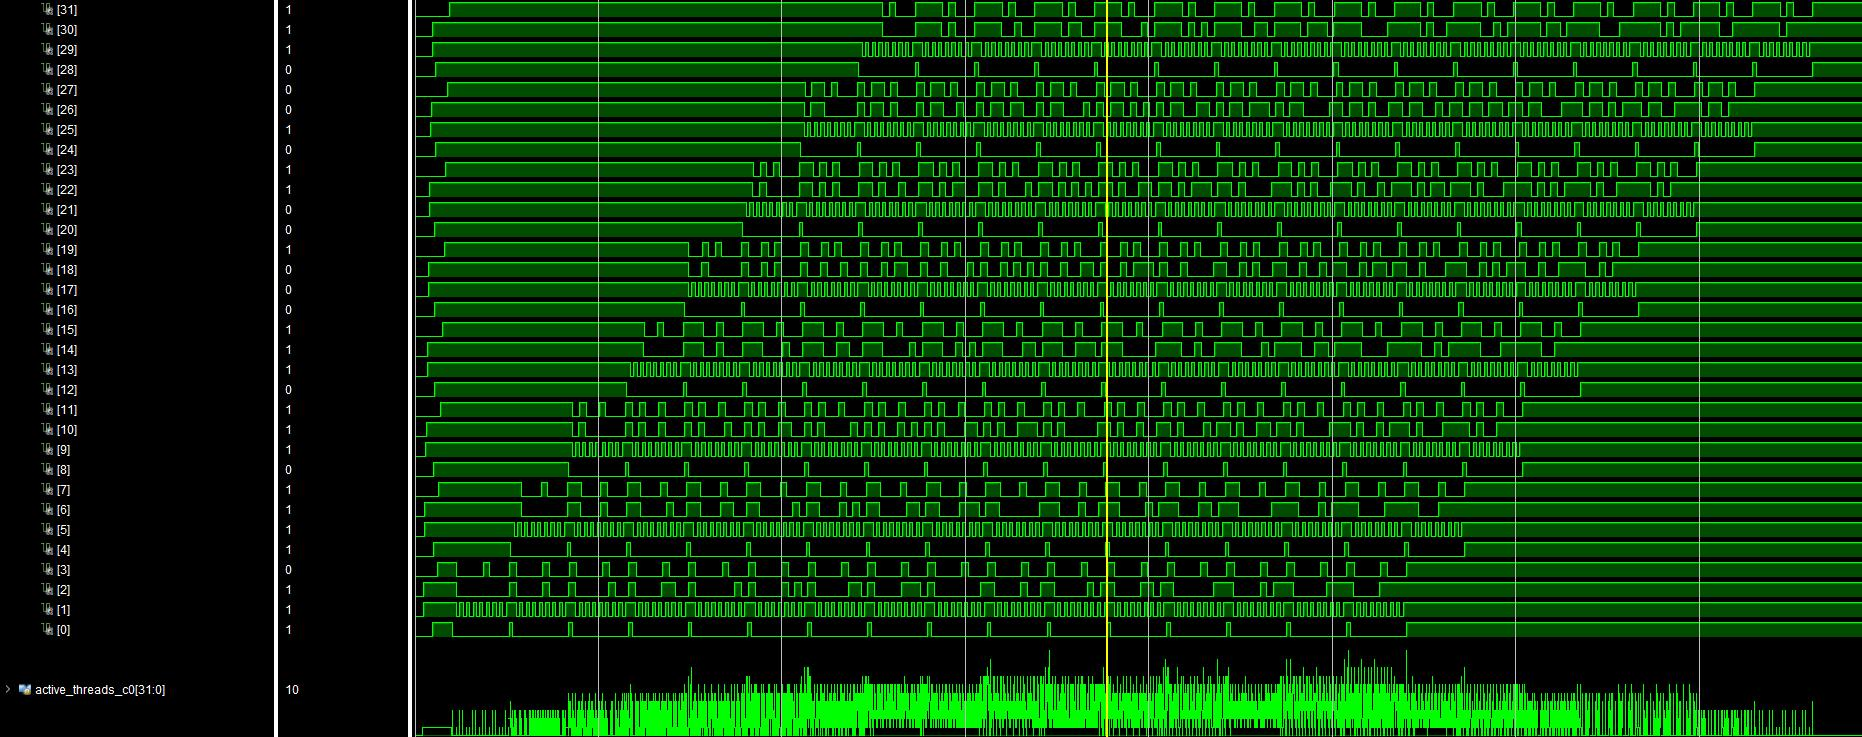
\includegraphics[width=6in]{figs/spi_threads}
	\caption{Running 8 SPI master and 8 SPI slave virtual peripherals from one core.}
	\label{spi_vp}
\end{figure*}

With this scheme in mind, we can now program virtual peripherals. A protocol is partitioned into individual timepoints, at which a protocol must be handled by a thread. For the time period, at which nothing needs to be done, the threads kills itself after it has programed the calendar to wake up a thread at a certain program location, which then continues with handling the program. Figure \ref{spi_vp} shows a demo simulation when running 8 SPI master and 8 SPI slave virtual peripherals on a single CUBE-V core. The bottom line shows the number of active threads, which is 10 at its peek. This is just one possibility to code virtual peripherals.

The current release contains initial versions of RS232 (115kBaud), I2C (50kHz) and SPI (25kHz) drivers. This is more of a prove of concept and is optimized to run 16 (15 in case of RS232) individual virtual peripherals at the same time on one core. The following improvements can be made in the future:

1) The provided drivers can be code-size and timing optimized. 

2) When equal or less than 4 threads (VPs) are running on a core, or when an exact number of threads (VPs) are running on a core, then the runtime of a thread is predictive, and the VPs could continuously execute the code (without being interrupted). This leads to higher baudrates.

3) When the design needs to support the master side of the protocol, multiple VPs can be executed in a parallel or sequential fashion. Parallel could mean for instance to extend the data width of an SPI to 5 bits to support 5 individual 1-bit SPIs. Sequential execution could mean, that in case the protocol does not need to be continuously driven, the serving of individual (and different) interfaces could alter accordingly.

Certainly one of the great benefits of such a software driven protocol is, that many custom ''or strange'' protocols variations are possible.
